\documentclass[../piano-di-progetto.tex]{subfiles}

\begin{document}

  \subsection{XI incremento}

  \subsubsection{Prospetto orario}
 Durante l'undicesimo incremento, la distribuzione oraria è la seguente:
  \begin{table}[H]
    \centering
    \begin{tabular}{lccccccc}
    \rowcolor{lightgray}
    \textbf{Nominativo}       & \textbf{Re} & \textbf{Am} & \textbf{An} & \textbf{Pt} & \textbf{Pr} & \textbf{Ve} & \textbf{Ore totali} \\
Sofia Bononi              & -          & 5           & -          & -          & -           & 6           & 11          \\
Enrico Buratto            & -          & -           & -          & 2          & 9           & 2           & 13          \\
Ian Nicolas Di Menna      & 4          & -           & -          & -          & -           & 6           & 10          \\
Alessandro Franchin       & -          & -           & -          & -          & 9           & 2           & 11          \\
Enrico Galdeman           & -          & -           & -          & -          & 9           & 4           & 13          \\
Nicholas Miazzo           & -          & 5           & -          & -          & -           & 5           & 10          \\
Marco Nardelotto          & -          & -           & -          & 4          & -           & 9           & 13          \\
\textbf{Ore totali ruolo} & \textbf{4} & \textbf{10} & \textbf{0} & \textbf{6} & \textbf{27} & \textbf{34} & \textbf{81}
    
    \end{tabular}
    \caption{Distribuzione oraria del undicesimo incremento}
  \end{table}


  Per facilitare la lettura della distribuzione oraria, i dati vengono rappresentati graficamente mediante il seguente istogramma:
  \begin{figure}[H]
    \centering
    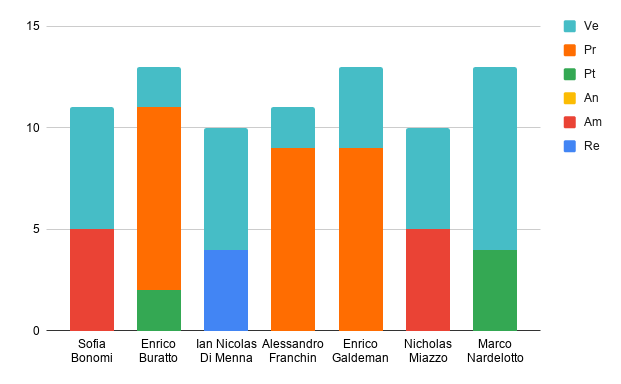
\includegraphics[width=12cm]{img/ore-11-incr.png}
    \caption{Istogramma della distribuzione oraria nel undicesimo incremento}
    \label{fig:ore-componente-progettazione}
  \end{figure}

  \subsubsection{Prospetto economico}
  In questo periodo, la suddivisione oraria e i costi per ruolo è la seguente:

  \begin{table}[H]
    \centering
    \begin{tabular}{lcc}
      \rowcolor{lightgray}
      \textbf{Ruolo}  & \textbf{Ore previste} & \textbf{Costo}      \\
Responsabile    & 4           & € 120,00            \\
Amministratore  & 10          & € 200,00            \\
Analista        & -           & € 0,00              \\
Progettista     & 6           & € 132,00            \\
Programmatore   & 27          & € 405,00            \\
Verificatore    & 34          & € 510,00            \\
\textbf{Totale} & \textbf{81} & \textbf{€ 1.367,00}
    \end{tabular}
    \caption{Prospetto economico nel undicesimo incremento}
  \end{table}


  Per facilitare la lettura della suddivisione oraria per ruolo, i dati vengono rappresentati graficamente mediante il seguente areogramma:
  \begin{figure}[H]
    \centering
    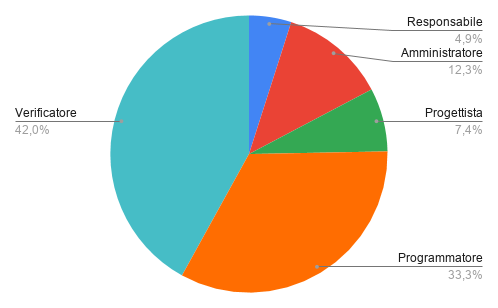
\includegraphics[width=12cm]{img/ruoli-11-incr.png}
    \caption{Areogramma della suddivisione dei ruoli nel undicesimo incremento}
    \label{fig:ore-ruolo-progettazione}
  \end{figure}



\end{document}
